\documentclass[a4paper,12pt]{article}
\usepackage[utf8]{inputenc}
\usepackage[english]{babel}
\usepackage{amsmath,amsfonts,amssymb}
\usepackage{graphicx}
\usepackage{caption}
\usepackage{hyperref}
\usepackage{geometry}
\usepackage{booktabs}
\usepackage[separate-uncertainty=true]{siunitx} % SI-Einheiten
\usepackage{float}
\usepackage[ISO]{diffcoeff} % Differentiale in hübsch
\usepackage{subcaption} % Bilder nebeneinander
\usepackage{wrapfig} % Bilder und Text zusammen
\usepackage{enumitem}
\usepackage{physics}

\geometry{left=2.5cm, right=2.5cm, top=2.5cm, bottom=2.5cm}

\title{Update: SIMBA in python}
\author{Stella Hoffmann}
\date{March}

\begin{document}

\maketitle

\tableofcontents

\newpage

\section{What I did}
\begin{figure}[H]
    \centering
    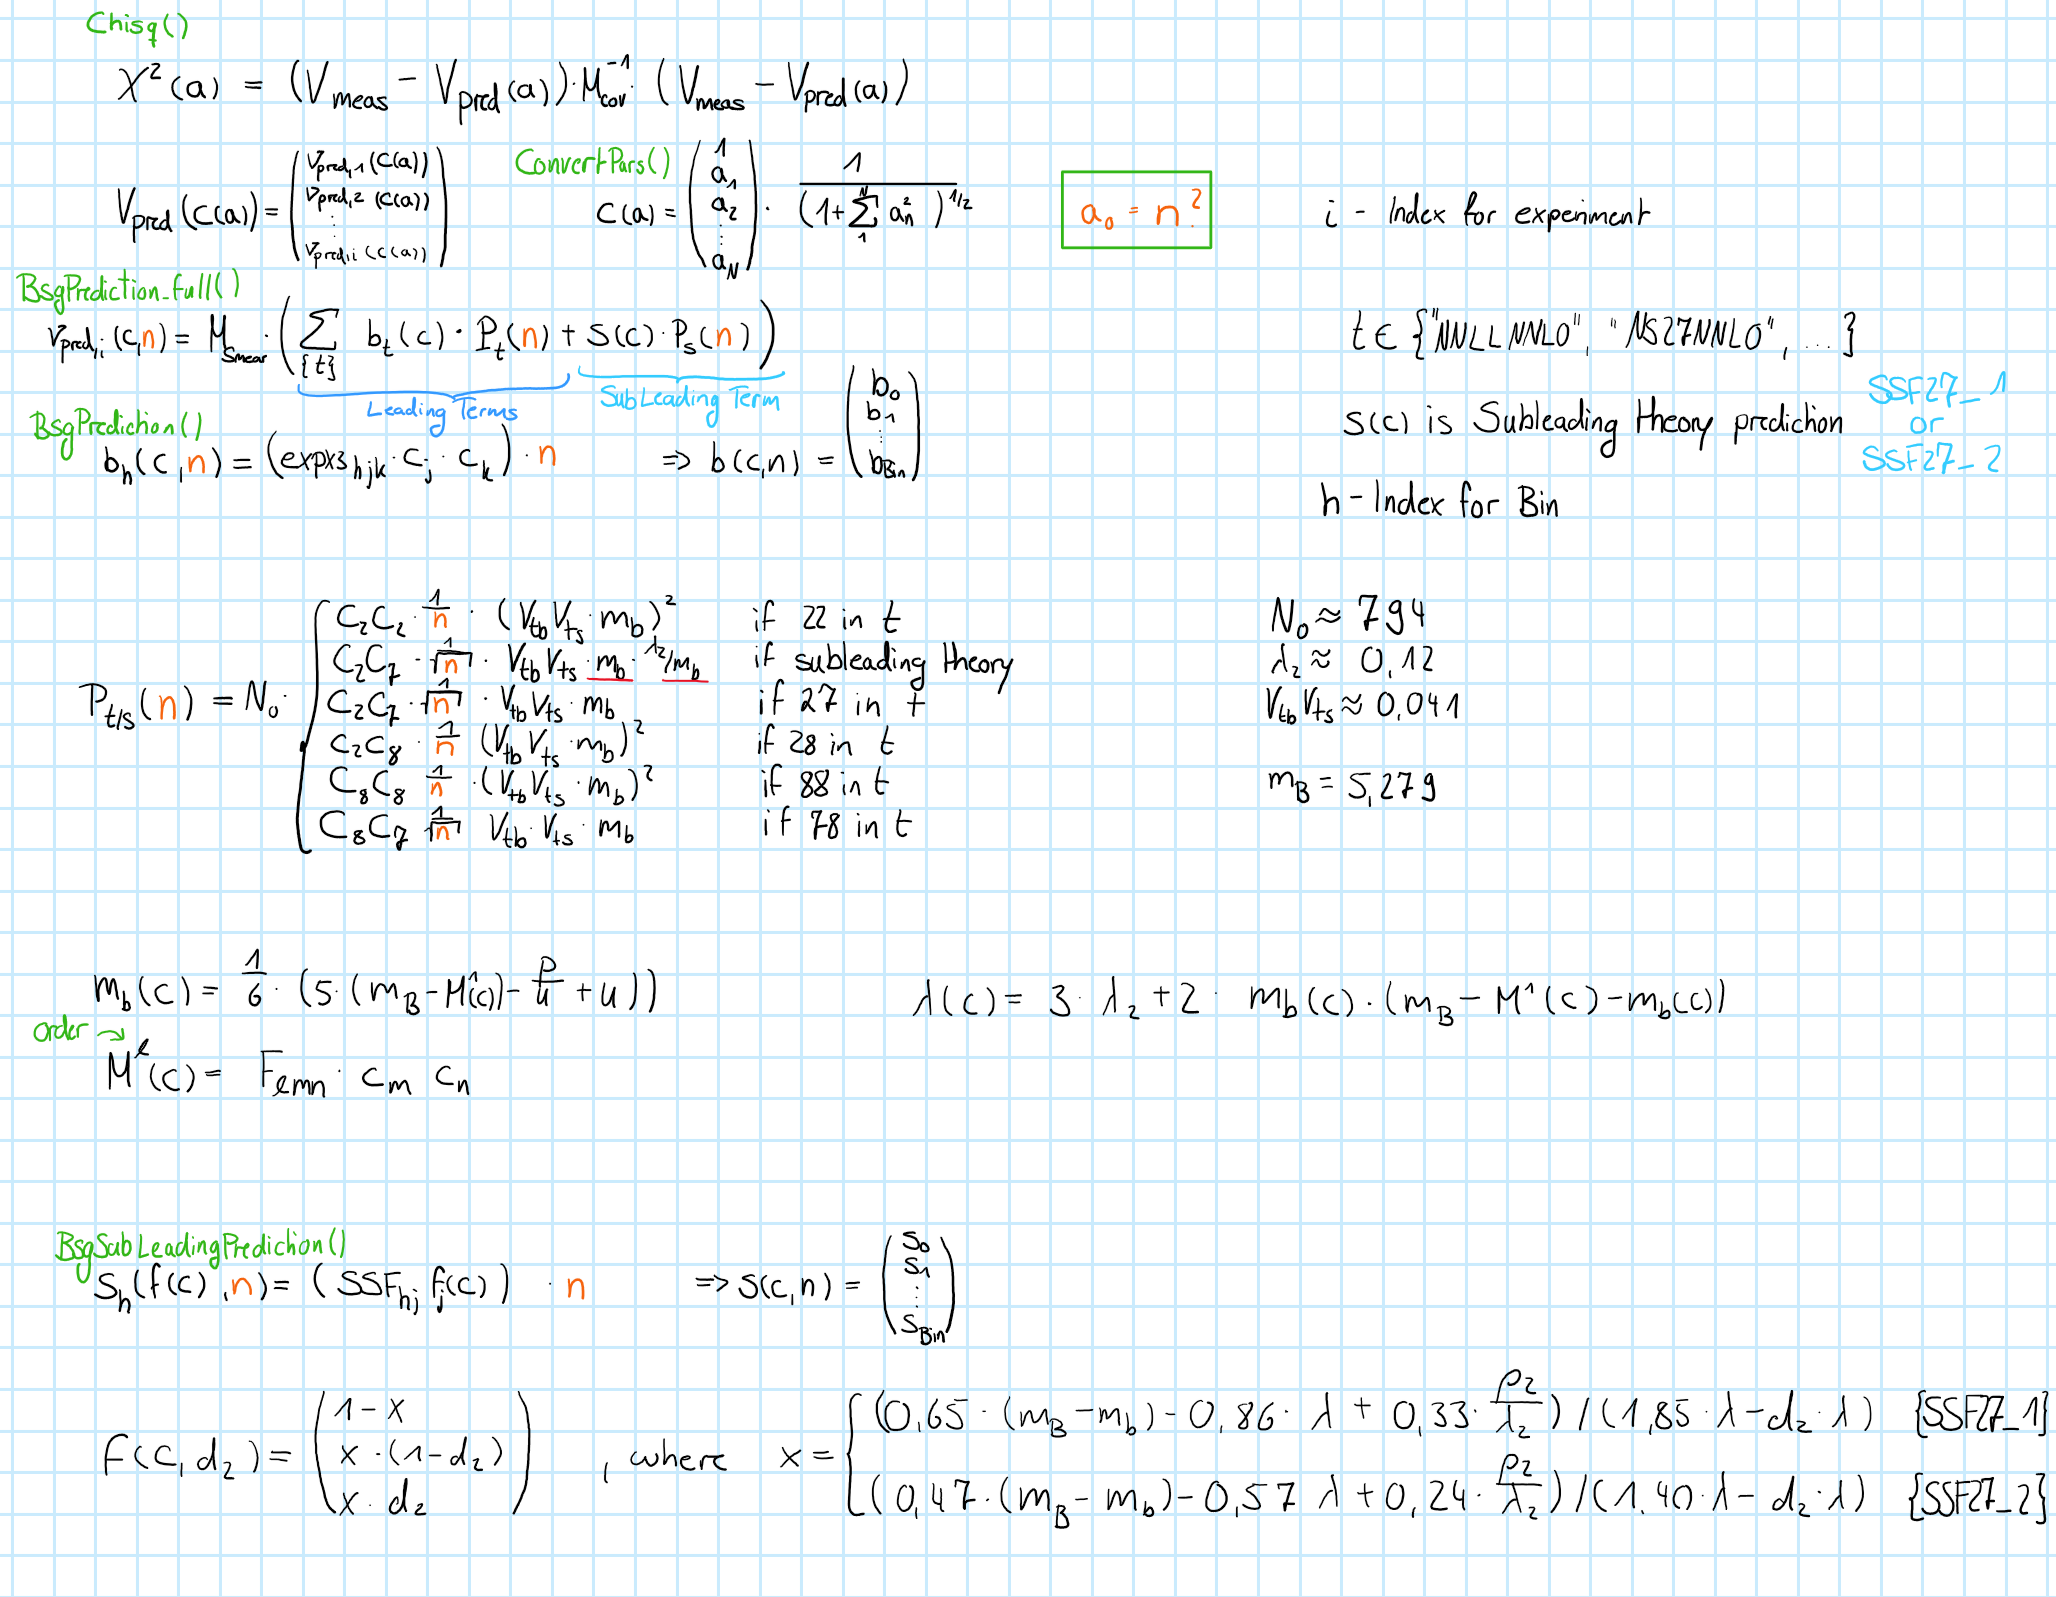
\includegraphics[scale=0.3]{equations.png}
    \caption{Equations according to my python code}
\end{figure}

A problem could be the $d_2$. In my code it's constantly zero. I got this information from the \textit{fit.config} file.
\begin{figure}[H]
    \centering
    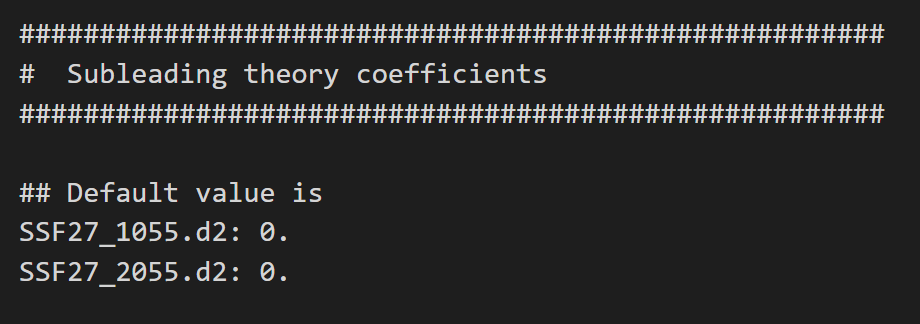
\includegraphics[scale=0.3]{d2_fit_config.png}
    \caption{Information in \textit{fit.config} file}
\end{figure}

\section{Comparisons}
As you can see in the following, something is off with the subleading theory. To compare different fits, I always plotted the Fit with the subleading prediction added on the leading prediction and with just the leading prediction.
For the fitting I used 4 to 7 start parameters, which gave different results for the prediction, as it is shown in the columns.
Every pair of rows has more amount of measurements included in the fit (\textit{["babar\_incl", "babar\_hadtag", "babar\_sem", "belle"]}).\\
The \textbf{red dots} show my calculated prediction.\\
The \textbf{black dots} show the experimental values, which I extracted from the root files.\\
The \textbf{green line} shows the fit I extracted from the root files.\\
The \textbf{blue line} shows the difference between the green line and the red dots.


\subsection{Babar hadronic tag}
\begin{figure}[H]
    \centering
    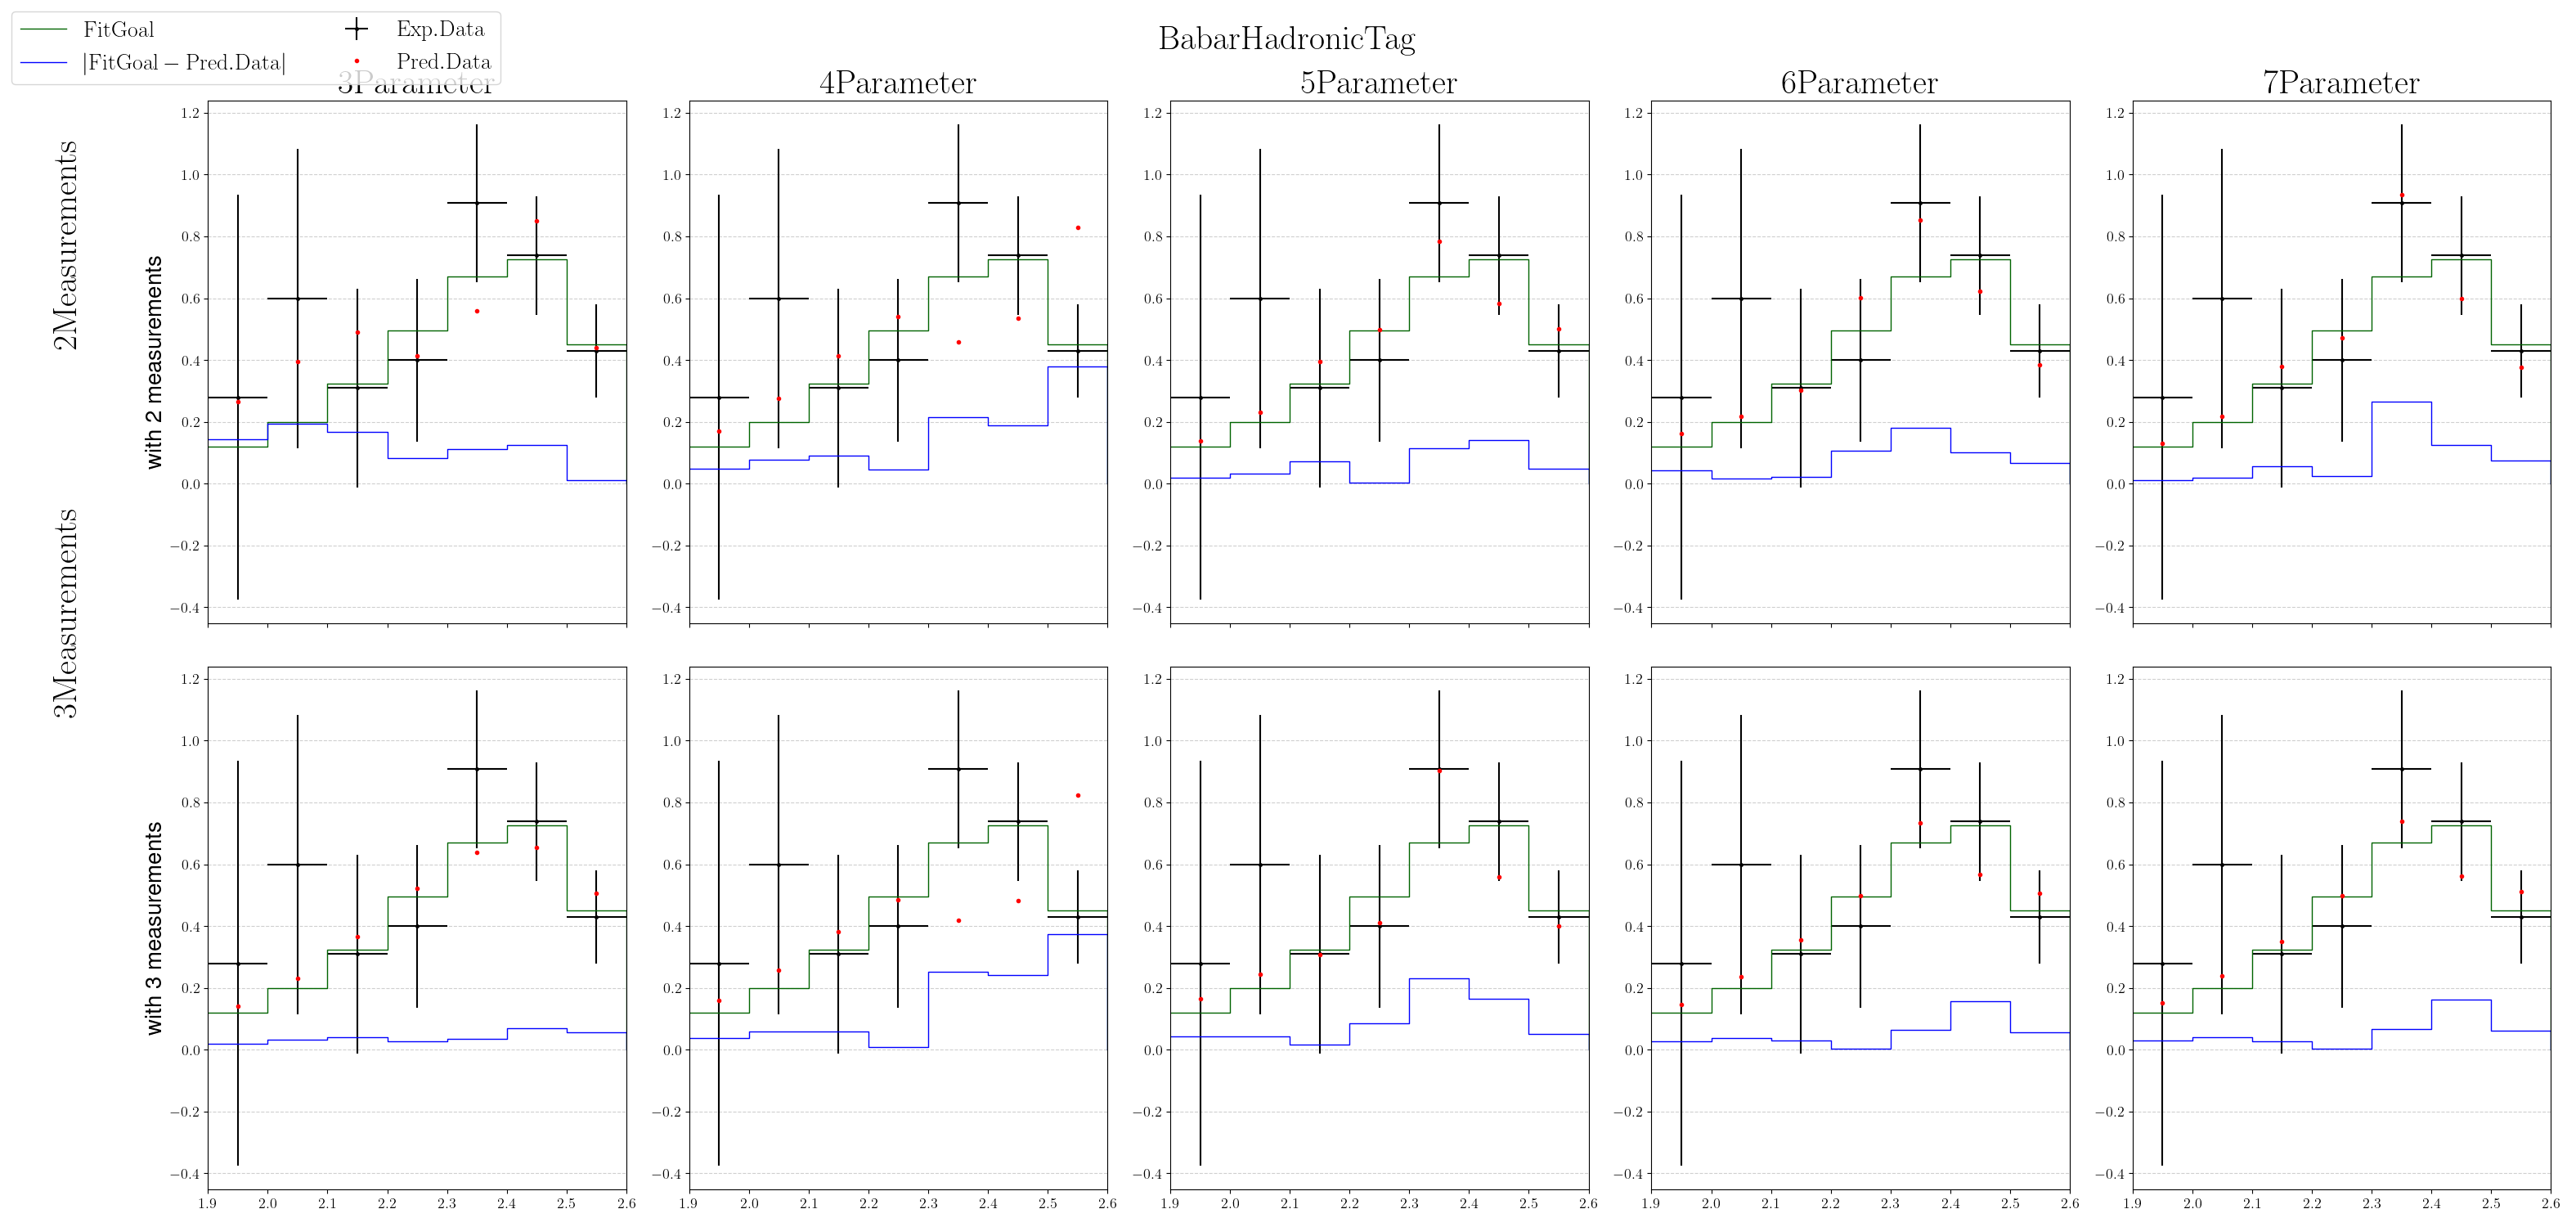
\includegraphics[scale=0.3]{../compare/babar_hadtag_soft_compare.png}
    \caption{Fit Comparison for 'babar\_hadtag'}
\end{figure}
\subsection{Babar inclusive spectra}
\begin{figure}[H]
    \centering
    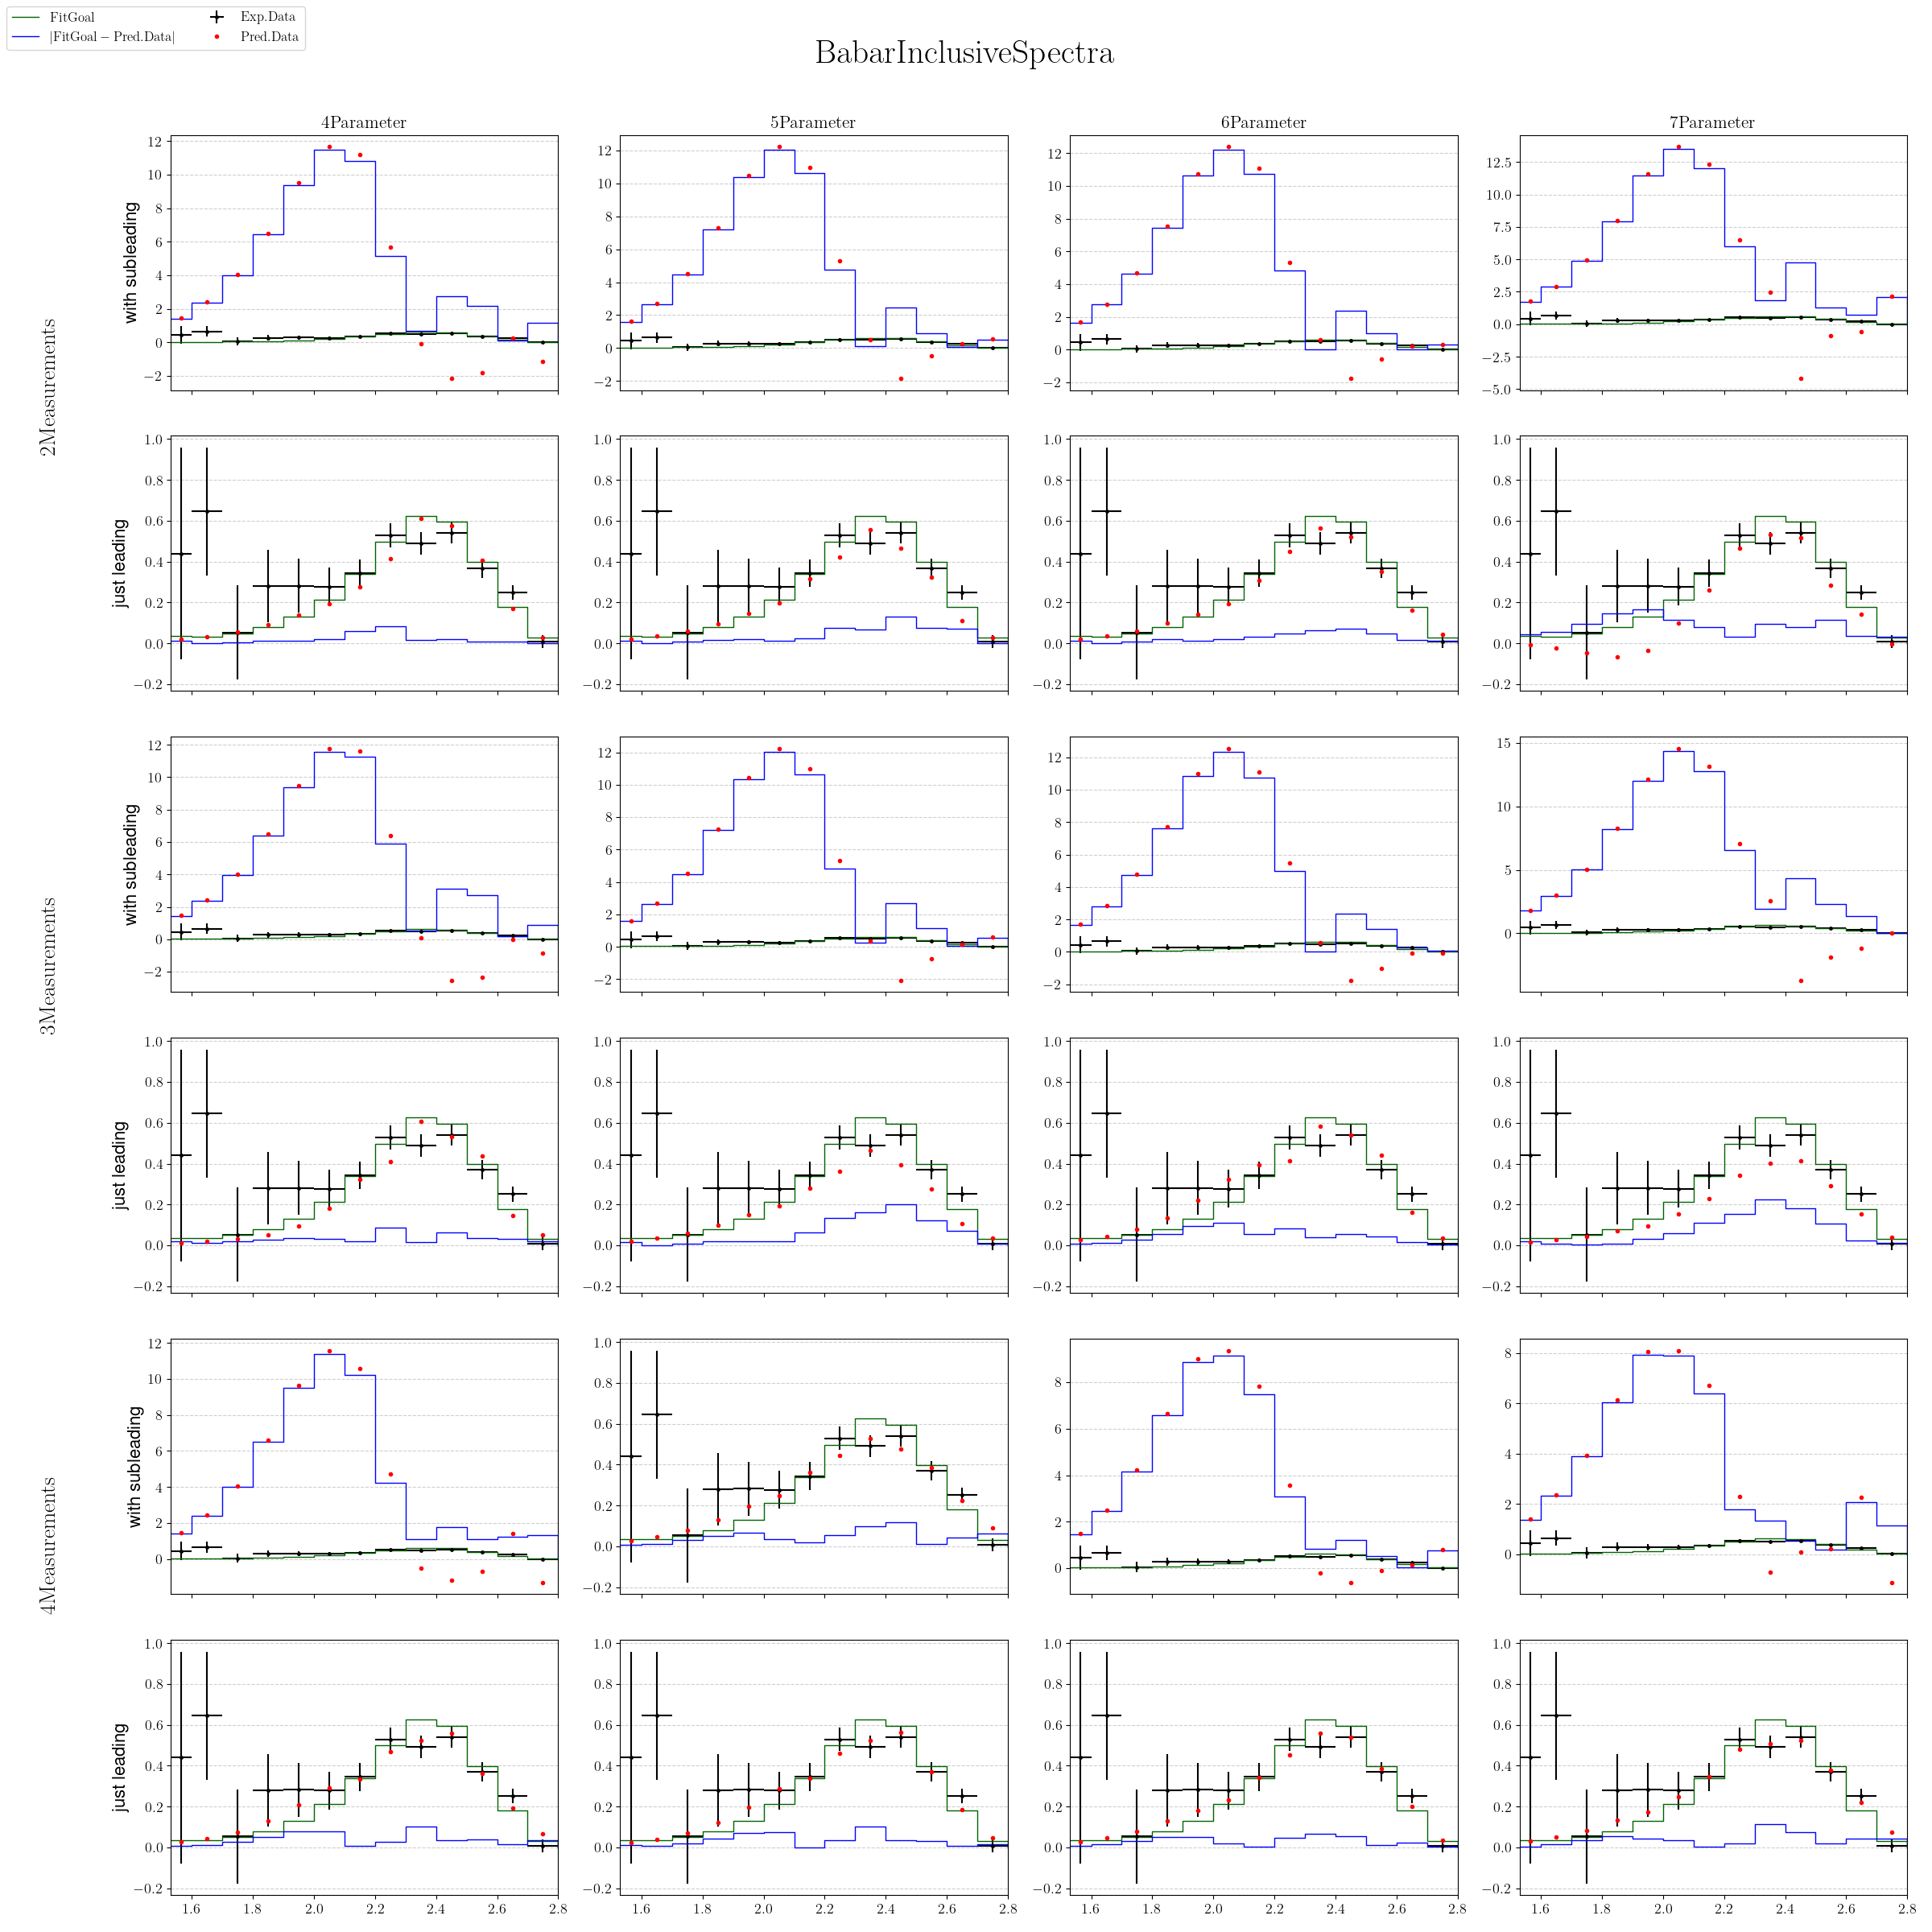
\includegraphics[scale=0.3]{../compare/babar_incl_soft_compare.png}
    \caption{Fit Comparison for 'babar\_incl'}
\end{figure}
\subsection{Babar semileptonic}
\begin{figure}[H]
    \centering
    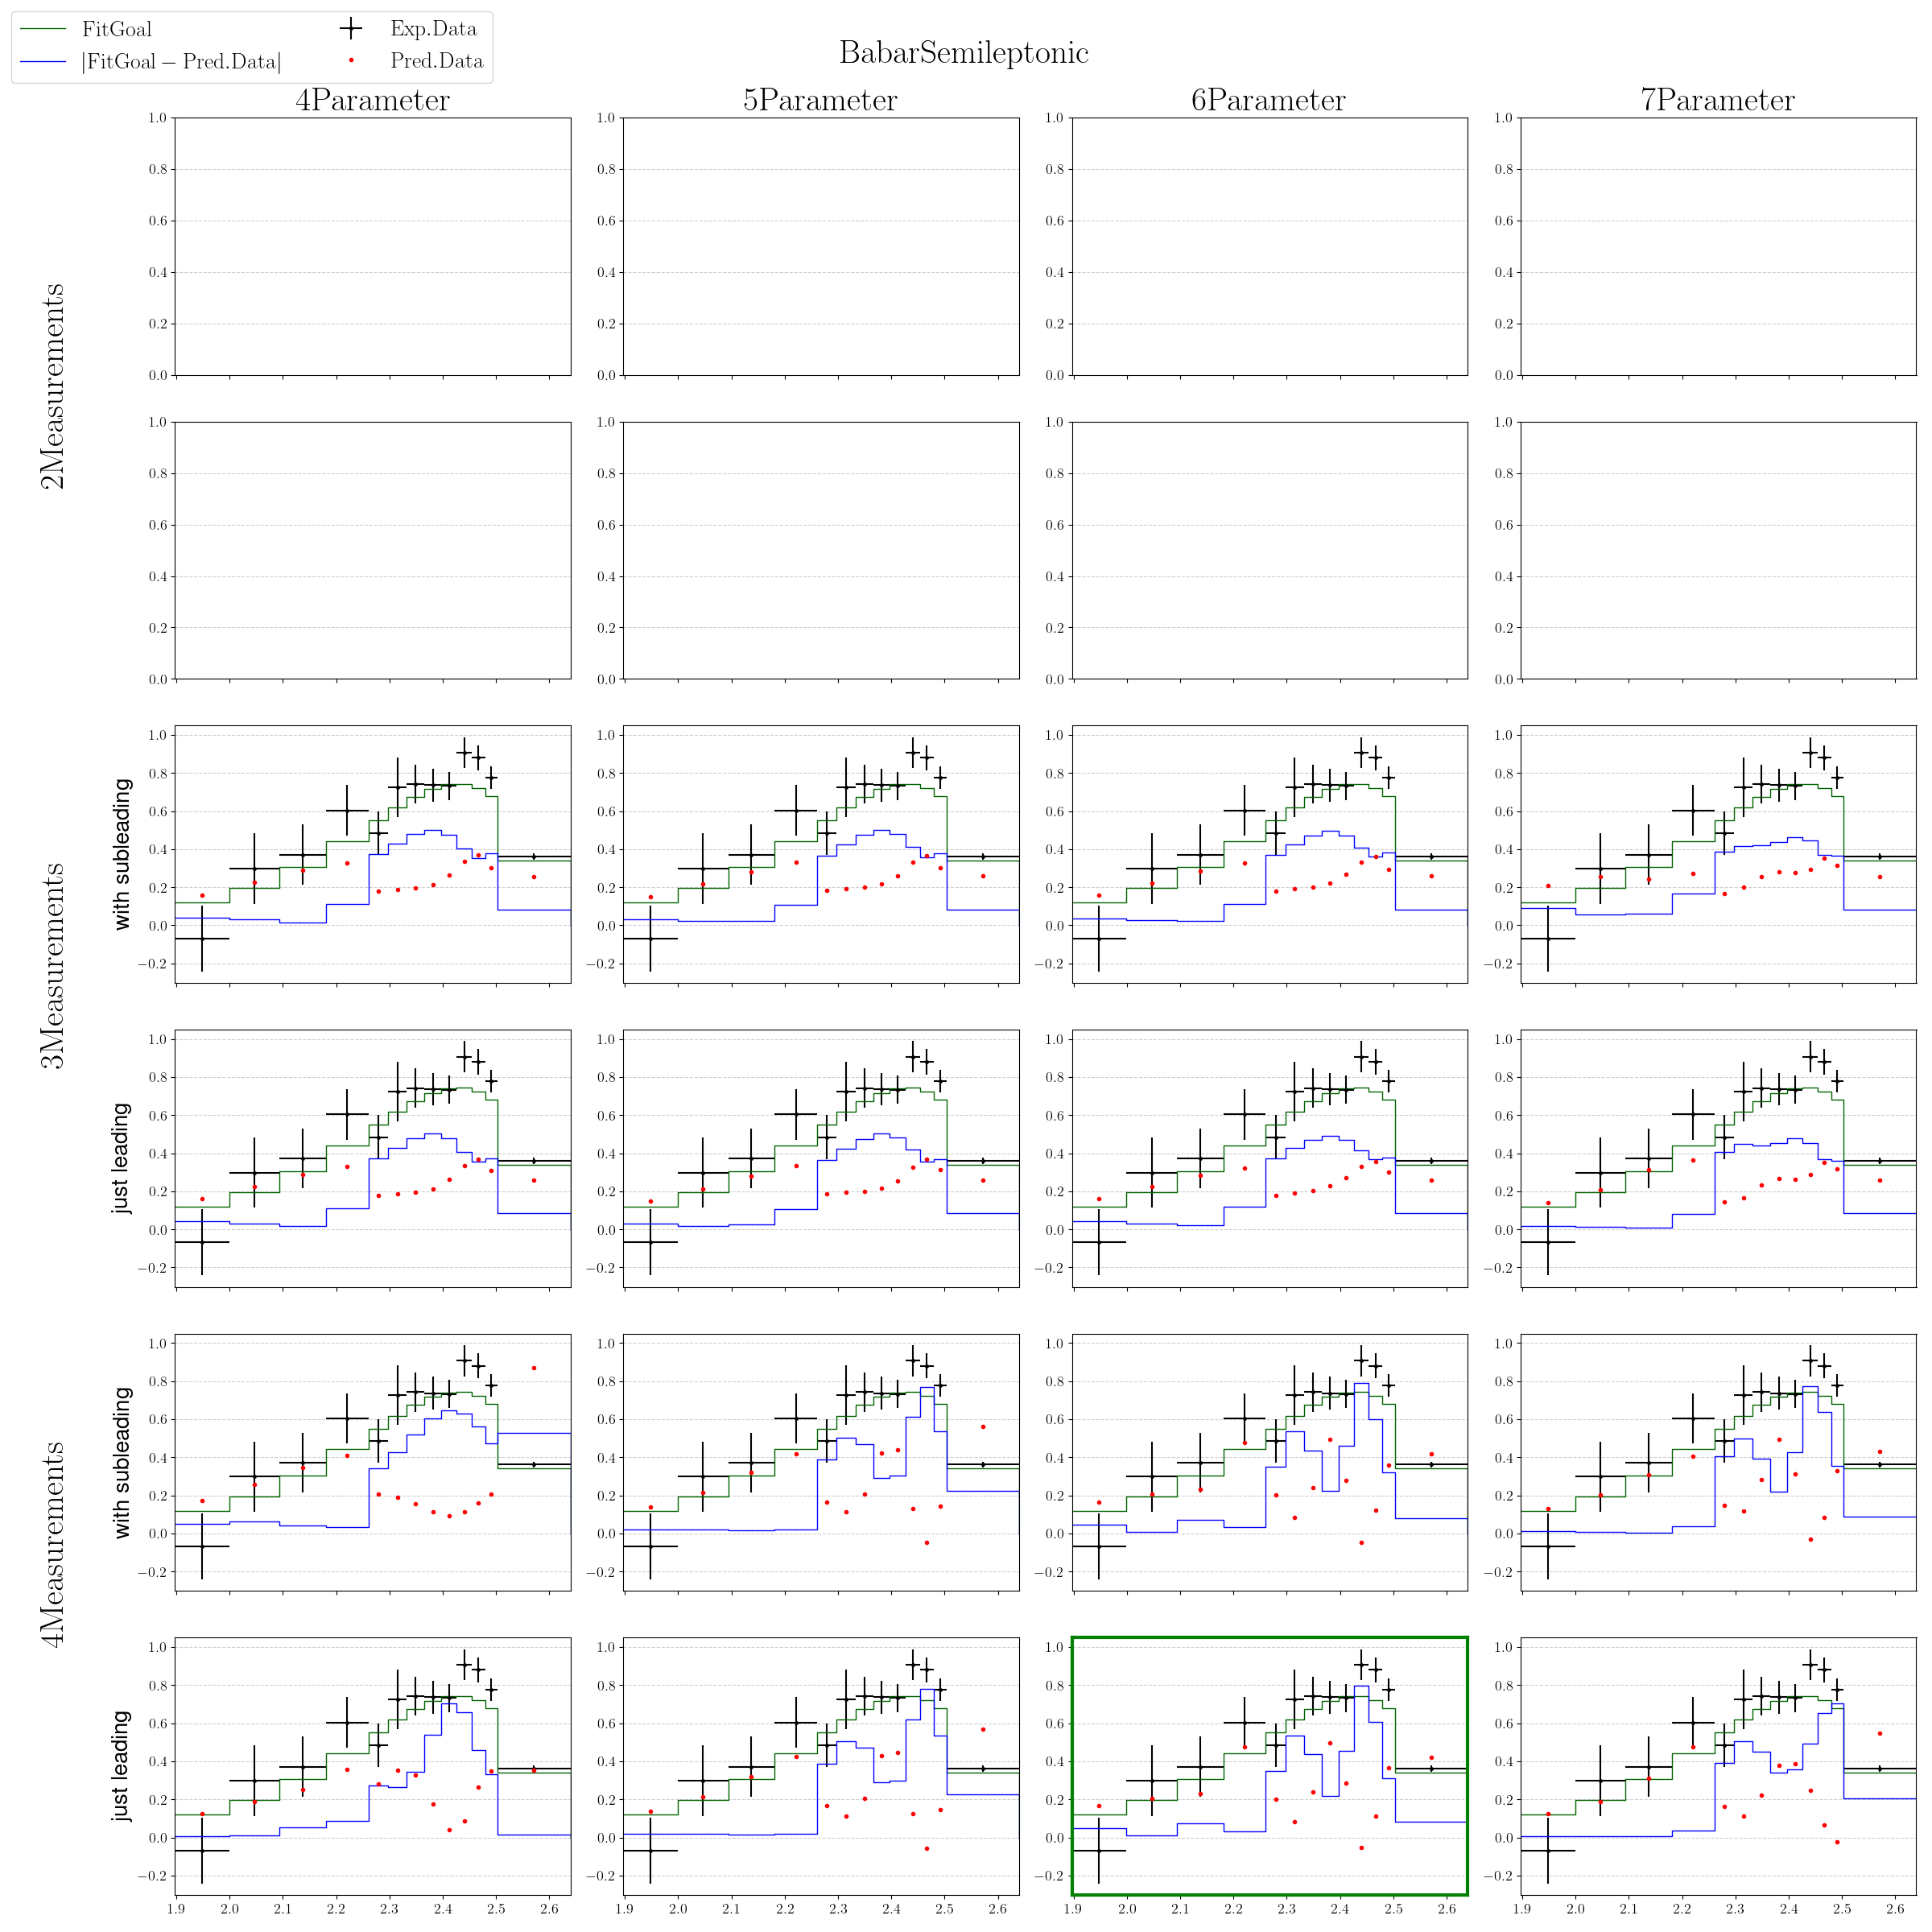
\includegraphics[scale=0.3]{../compare/babar_sem_soft_compare.png}
    \caption{Fit Comparison for 'babar\_sem'}
\end{figure}
\subsection{Belle}
\begin{figure}[H]
    \centering
    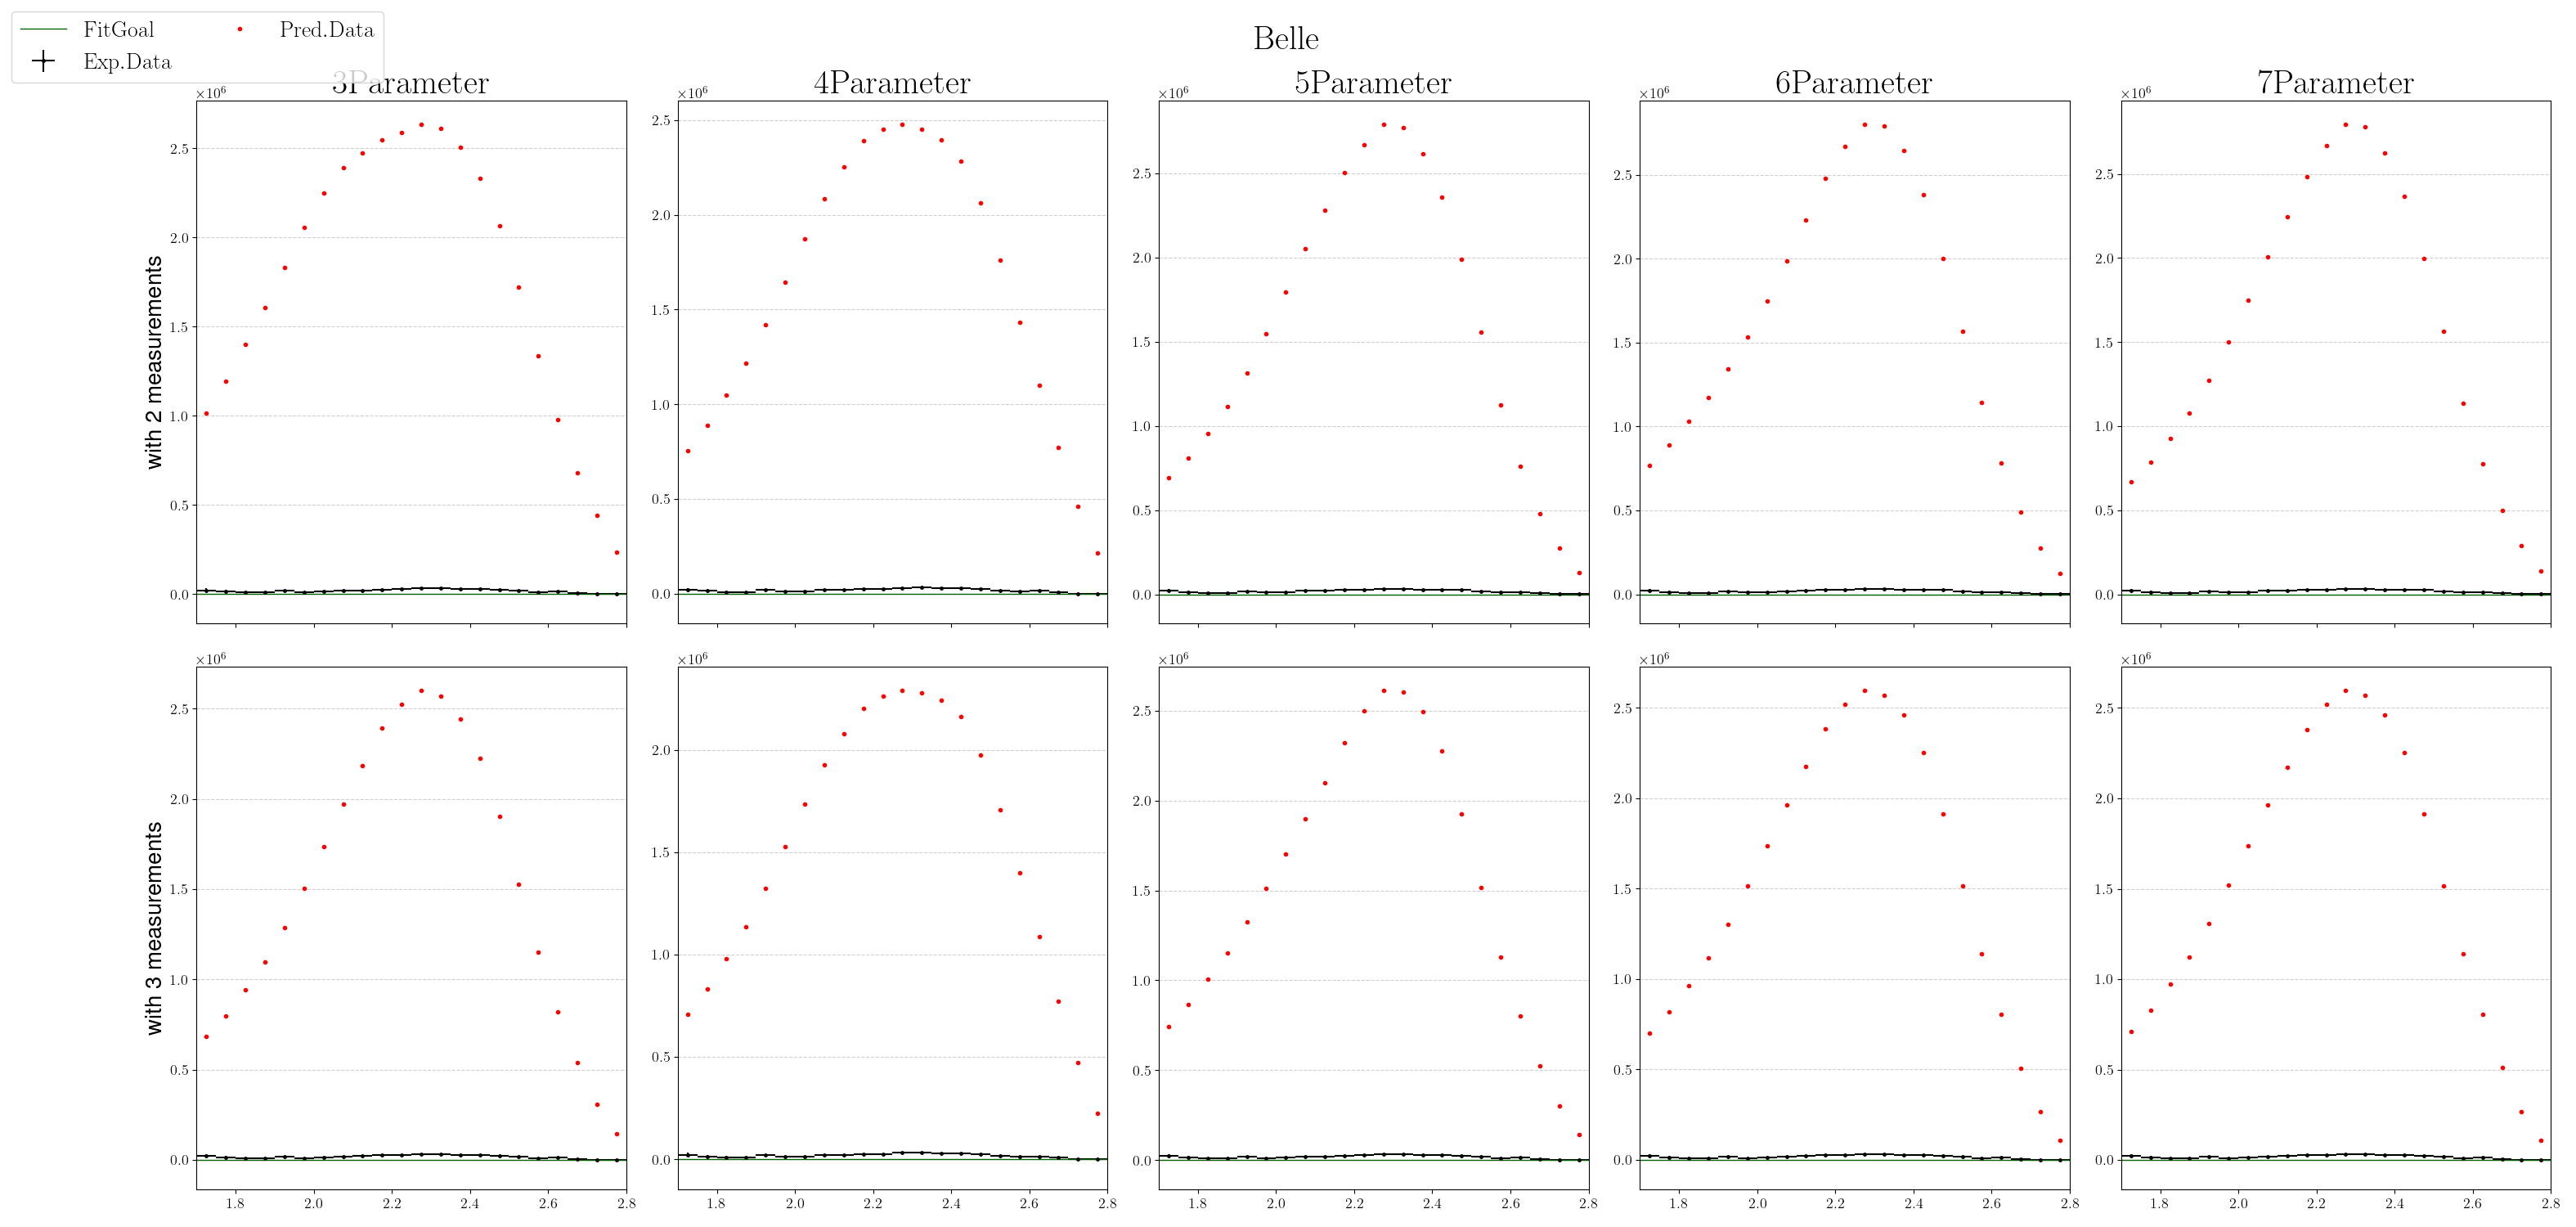
\includegraphics[scale=0.3]{../compare/belle_soft_compare.png}
    \caption{Fit Comparison for 'belle'}
\end{figure}

\end{document}